% =============================================================================
% Appendix J: Message Sequence Diagrams
% תרשימי רצף הודעות
% Standalone chapter with subfiles support
% =============================================================================

\documentclass[../master/main.tex]{subfiles}

\begin{document}

\chapter*{נספח י': תרשימי רצף הודעות}
\addcontentsline{toc}{chapter}{נספח י': תרשימי רצף הודעות}
\renewcommand{\thehebrewsection}{י.\arabic{hebrewsection}}
\setcounter{hebrewsection}{0}

\par\needspace{5\baselineskip}
\hebrewsection{מבוא}

נספח זה מציג תרשימי רצף (\en{Sequence Diagrams}) עבור התרחישים העיקריים במערכת. התרשימים מדגימים את סדר ההודעות בין הסוכנים לבין מנהל הליגה.

% =============================================================================
\par\needspace{5\baselineskip}
\hebrewsection{רצף רישום לליגה}
\label{sec:seq-registration}
% =============================================================================

\begin{figure}[htbp]
\centering
\begin{english}
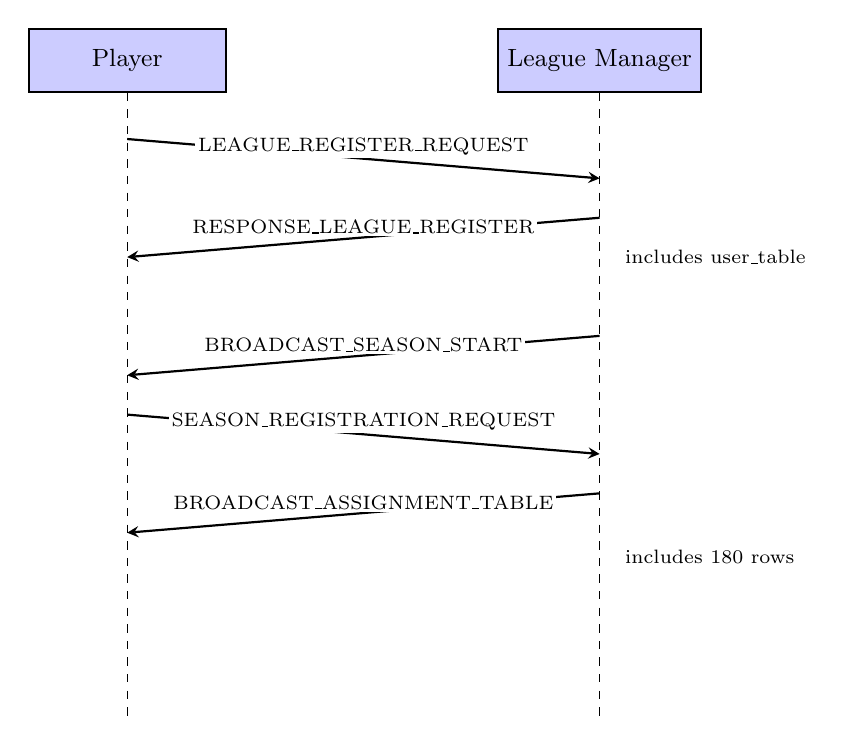
\begin{tikzpicture}[
    actor/.style={rectangle, draw, thick, fill=blue!20, minimum width=2.5cm, minimum height=0.8cm, font=\small},
    msg/.style={->, thick, >=stealth},
    msglabel/.style={font=\scriptsize, fill=white, inner sep=1pt}
]
    % Actors
    \node[actor] (player) at (0,0) {Player};
    \node[actor] (lgm) at (6,0) {League Manager};

    % Lifelines
    \draw[dashed] (player.south) -- ++(0,-8);
    \draw[dashed] (lgm.south) -- ++(0,-8);

    % Messages
    \draw[msg] (0,-1) -- (6,-1.5) node[msglabel, midway, above] {LEAGUE\_REGISTER\_REQUEST};
    \draw[msg] (6,-2) -- (0,-2.5) node[msglabel, midway, above] {RESPONSE\_LEAGUE\_REGISTER};
    \draw[msg] (6,-3.5) -- (0,-4) node[msglabel, midway, above] {BROADCAST\_SEASON\_START};
    \draw[msg] (0,-4.5) -- (6,-5) node[msglabel, midway, above] {SEASON\_REGISTRATION\_REQUEST};
    \draw[msg] (6,-5.5) -- (0,-6) node[msglabel, midway, above] {BROADCAST\_ASSIGNMENT\_TABLE};

    % Notes
    \node[font=\scriptsize, right] at (6.2,-2.5) {includes user\_table};
    \node[font=\scriptsize, right] at (6.2,-6.3) {includes 180 rows};

\end{tikzpicture}
\end{english}
\caption{רצף רישום שחקן לליגה ולעונה}
\label{fig:seq-registration}
\end{figure}

% =============================================================================
\par\needspace{5\baselineskip}
\hebrewsection{רצף תחילת עונה}
\label{sec:seq-season-start}
% =============================================================================

\begin{figure}[htbp]
\centering
\begin{english}
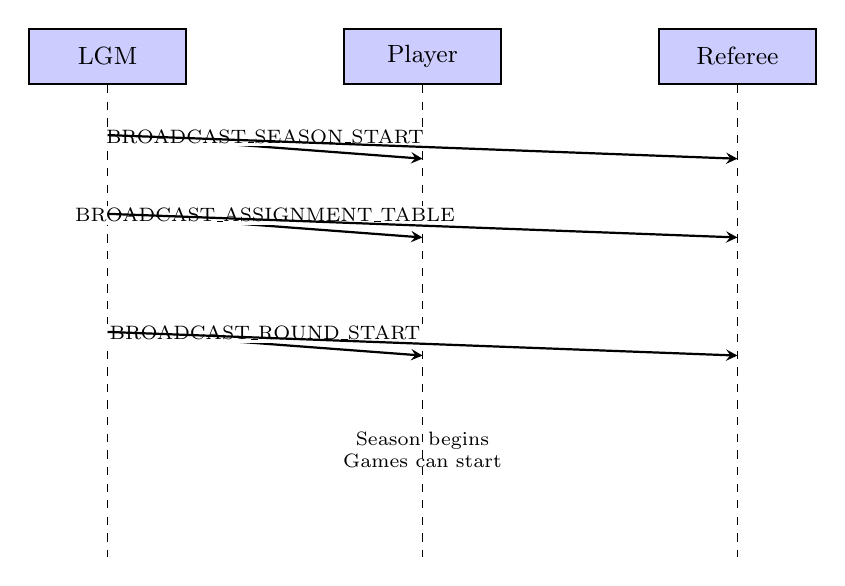
\begin{tikzpicture}[
    actor/.style={rectangle, draw, thick, fill=blue!20, minimum width=2cm, minimum height=0.7cm, font=\small},
    msg/.style={->, thick, >=stealth},
    msglabel/.style={font=\scriptsize, fill=white, inner sep=1pt}
]
    % Actors
    \node[actor] (lgm) at (0,0) {LGM};
    \node[actor] (player) at (4,0) {Player};
    \node[actor] (referee) at (8,0) {Referee};

    % Lifelines
    \draw[dashed] (lgm.south) -- ++(0,-6);
    \draw[dashed] (player.south) -- ++(0,-6);
    \draw[dashed] (referee.south) -- ++(0,-6);

    % Broadcasts (to both)
    \draw[msg] (0,-1) -- (4,-1.3) node[msglabel, midway, above] {BROADCAST\_SEASON\_START};
    \draw[msg] (0,-1) -- (8,-1.3);

    \draw[msg] (0,-2) -- (4,-2.3) node[msglabel, midway, above] {BROADCAST\_ASSIGNMENT\_TABLE};
    \draw[msg] (0,-2) -- (8,-2.3);

    \draw[msg] (0,-3.5) -- (4,-3.8) node[msglabel, midway, above] {BROADCAST\_ROUND\_START};
    \draw[msg] (0,-3.5) -- (8,-3.8);

    % Note
    \node[font=\scriptsize, text width=3cm, align=center] at (4,-5) {Season begins\\Games can start};

\end{tikzpicture}
\end{english}
\caption{רצף התחלת עונה}
\label{fig:seq-season-start}
\end{figure}

% =============================================================================
\par\needspace{5\baselineskip}
\hebrewsection{רצף משחק מלא}
\label{sec:seq-full-game}
% =============================================================================

\begin{figure}[htbp]
\centering
\begin{english}
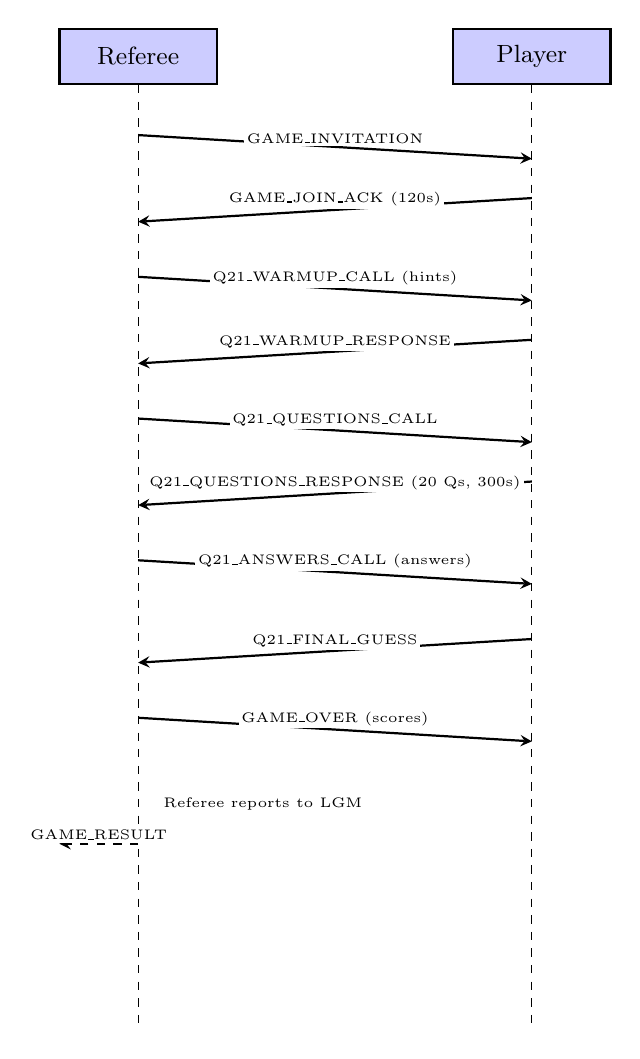
\begin{tikzpicture}[
    actor/.style={rectangle, draw, thick, fill=blue!20, minimum width=2cm, minimum height=0.7cm, font=\small},
    msg/.style={->, thick, >=stealth},
    msglabel/.style={font=\tiny, fill=white, inner sep=1pt}
]
    % Actors
    \node[actor] (referee) at (0,0) {Referee};
    \node[actor] (player) at (5,0) {Player};

    % Lifelines
    \draw[dashed] (referee.south) -- ++(0,-12);
    \draw[dashed] (player.south) -- ++(0,-12);

    % Game invitation
    \draw[msg] (0,-1) -- (5,-1.3) node[msglabel, midway, above] {GAME\_INVITATION};
    \draw[msg] (5,-1.8) -- (0,-2.1) node[msglabel, midway, above] {GAME\_JOIN\_ACK (120s)};

    % Warmup
    \draw[msg] (0,-2.8) -- (5,-3.1) node[msglabel, midway, above] {Q21\_WARMUP\_CALL (hints)};
    \draw[msg] (5,-3.6) -- (0,-3.9) node[msglabel, midway, above] {Q21\_WARMUP\_RESPONSE};

    % Questions
    \draw[msg] (0,-4.6) -- (5,-4.9) node[msglabel, midway, above] {Q21\_QUESTIONS\_CALL};
    \draw[msg] (5,-5.4) -- (0,-5.7) node[msglabel, midway, above] {Q21\_QUESTIONS\_RESPONSE (20 Qs, 300s)};

    % Answers
    \draw[msg] (0,-6.4) -- (5,-6.7) node[msglabel, midway, above] {Q21\_ANSWERS\_CALL (answers)};

    % Final guess
    \draw[msg] (5,-7.4) -- (0,-7.7) node[msglabel, midway, above] {Q21\_FINAL\_GUESS};

    % Game over
    \draw[msg] (0,-8.4) -- (5,-8.7) node[msglabel, midway, above] {GAME\_OVER (scores)};

    % Report to LGM
    \node[font=\tiny, right] at (0.2,-9.5) {Referee reports to LGM};
    \draw[msg, dashed] (0,-10) -- ++(-1,0) node[msglabel, midway, above] {GAME\_RESULT};

\end{tikzpicture}
\end{english}
\caption{רצף משחק \en{Q21} מלא}
\label{fig:seq-full-game}
\end{figure}

% =============================================================================
\par\needspace{5\baselineskip}
\hebrewsection{רצף תגובה לשידור}
\label{sec:seq-broadcast-response}
% =============================================================================

\begin{figure}[htbp]
\centering
\begin{english}
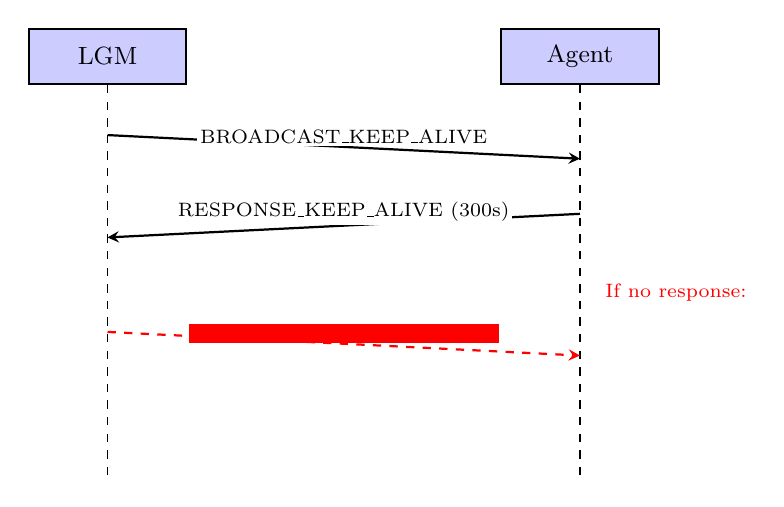
\begin{tikzpicture}[
    actor/.style={rectangle, draw, thick, fill=blue!20, minimum width=2cm, minimum height=0.7cm, font=\small},
    msg/.style={->, thick, >=stealth},
    msglabel/.style={font=\scriptsize, fill=white, inner sep=1pt}
]
    % Actors
    \node[actor] (lgm) at (0,0) {LGM};
    \node[actor] (agent) at (6,0) {Agent};

    % Lifelines
    \draw[dashed] (lgm.south) -- ++(0,-5);
    \draw[dashed] (agent.south) -- ++(0,-5);

    % Broadcast requiring response
    \draw[msg] (0,-1) -- (6,-1.3) node[msglabel, midway, above] {BROADCAST\_KEEP\_ALIVE};
    \draw[msg] (6,-2) -- (0,-2.3) node[msglabel, midway, above] {RESPONSE\_KEEP\_ALIVE (300s)};

    % Notes
    \node[font=\scriptsize, right, red] at (6.2,-3) {If no response:};
    \draw[msg, red, dashed] (0,-3.5) -- (6,-3.8) node[msglabel, midway, above, red] {REJECTION\_NOTIFICATION};

\end{tikzpicture}
\end{english}
\caption{רצף תגובה לשידור (עם מועד)}
\label{fig:seq-broadcast}
\end{figure}

% =============================================================================
\par\needspace{5\baselineskip}
\hebrewsection{רצף בקשת הארכה}
\label{sec:seq-extension}
% =============================================================================

\begin{figure}[htbp]
\centering
\begin{english}
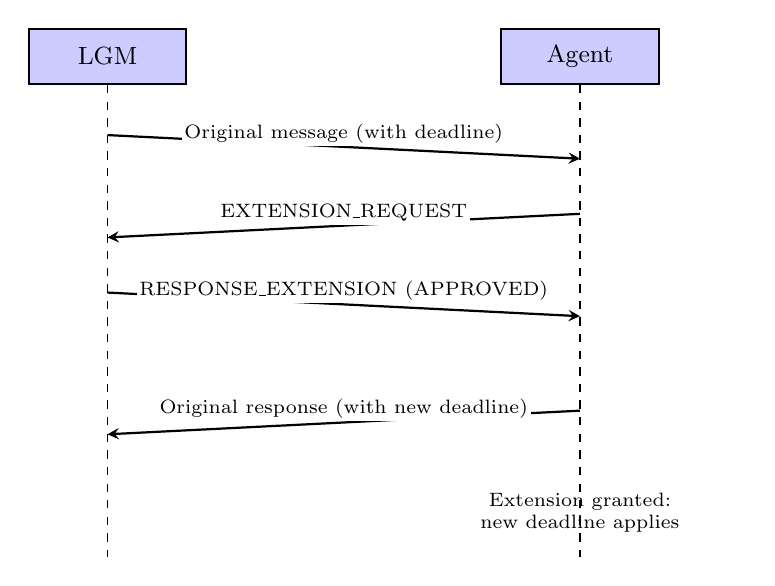
\begin{tikzpicture}[
    actor/.style={rectangle, draw, thick, fill=blue!20, minimum width=2cm, minimum height=0.7cm, font=\small},
    msg/.style={->, thick, >=stealth},
    msglabel/.style={font=\scriptsize, fill=white, inner sep=1pt}
]
    % Actors
    \node[actor] (lgm) at (0,0) {LGM};
    \node[actor] (agent) at (6,0) {Agent};

    % Lifelines
    \draw[dashed] (lgm.south) -- ++(0,-6);
    \draw[dashed] (agent.south) -- ++(0,-6);

    % Original message
    \draw[msg] (0,-1) -- (6,-1.3) node[msglabel, midway, above] {Original message (with deadline)};

    % Extension request (before deadline!)
    \draw[msg] (6,-2) -- (0,-2.3) node[msglabel, midway, above] {EXTENSION\_REQUEST};
    \draw[msg] (0,-3) -- (6,-3.3) node[msglabel, midway, above] {RESPONSE\_EXTENSION (APPROVED)};

    % Response with new deadline
    \draw[msg] (6,-4.5) -- (0,-4.8) node[msglabel, midway, above] {Original response (with new deadline)};

    % Note
    \node[font=\scriptsize, text width=4cm, align=center] at (6,-5.8) {Extension granted:\\new deadline applies};

\end{tikzpicture}
\end{english}
\caption{רצף בקשת הארכה מוצלחת}
\label{fig:seq-extension}
\end{figure}

% =============================================================================
\par\needspace{5\baselineskip}
\hebrewsection{רצף כוח עליון}
\label{sec:seq-force-majeure}
% =============================================================================

\begin{figure}[htbp]
\centering
\begin{english}
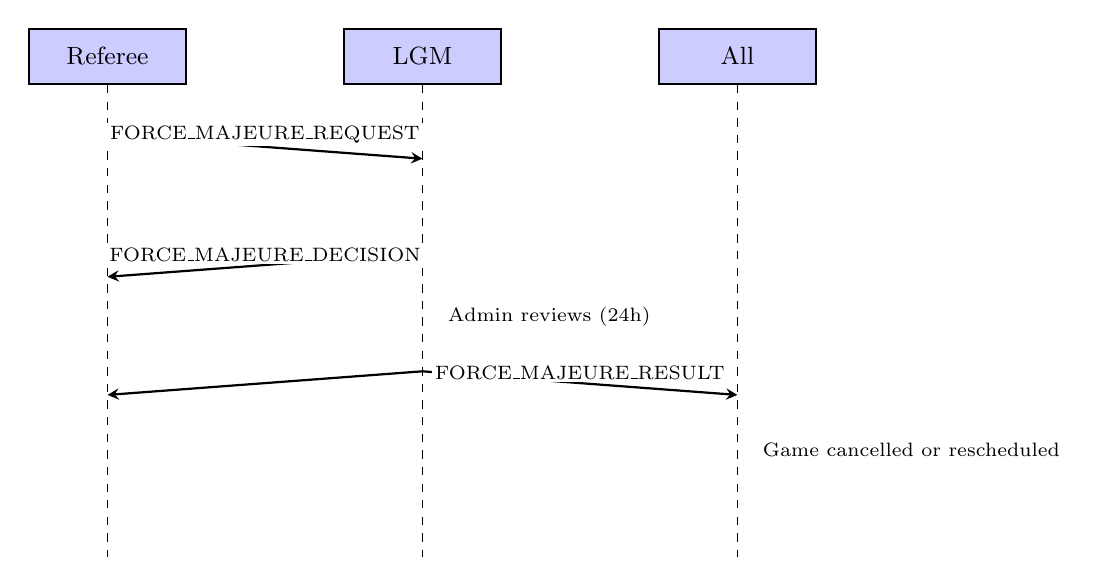
\begin{tikzpicture}[
    actor/.style={rectangle, draw, thick, fill=blue!20, minimum width=2cm, minimum height=0.7cm, font=\small},
    msg/.style={->, thick, >=stealth},
    msglabel/.style={font=\scriptsize, fill=white, inner sep=1pt}
]
    % Actors
    \node[actor] (ref) at (0,0) {Referee};
    \node[actor] (lgm) at (4,0) {LGM};
    \node[actor] (all) at (8,0) {All};

    % Lifelines
    \draw[dashed] (ref.south) -- ++(0,-6);
    \draw[dashed] (lgm.south) -- ++(0,-6);
    \draw[dashed] (all.south) -- ++(0,-6);

    % Force majeure flow
    \draw[msg] (0,-1) -- (4,-1.3) node[msglabel, midway, above] {FORCE\_MAJEURE\_REQUEST};
    \draw[msg] (4,-2.5) -- (0,-2.8) node[msglabel, midway, above] {FORCE\_MAJEURE\_DECISION};
    \draw[msg] (4,-4) -- (8,-4.3) node[msglabel, midway, above] {FORCE\_MAJEURE\_RESULT};
    \draw[msg] (4,-4) -- (0,-4.3);

    % Notes
    \node[font=\scriptsize, right] at (4.2,-3.3) {Admin reviews (24h)};
    \node[font=\scriptsize, right] at (8.2,-5) {Game cancelled or rescheduled};

\end{tikzpicture}
\end{english}
\caption{רצף בקשת כוח עליון}
\label{fig:seq-force-majeure}
\end{figure}

% =============================================================================
\par\needspace{5\baselineskip}
\hebrewsection{סיכום מועדי תגובה}
\label{sec:deadline-summary}
% =============================================================================

\begin{fancytable}{lcc}{מועדי תגובה לפי הודעה}
\label{tab:response-deadlines}
הודעה מקורית & מועד תגובה & הודעת תגובה \\
\en{GAME\_INVITATION} & \en{120s} & \en{GAME\_JOIN\_ACK} \\
\en{Q21\_WARMUP\_CALL} & \en{120s} & \en{Q21\_WARMUP\_RESPONSE} \\
\en{Q21\_QUESTIONS\_CALL} & \en{300s} & \en{Q21\_QUESTIONS\_RESPONSE} \\
\en{BROADCAST\_CONNECTIVITY\_TEST} & \en{60s} & \en{RESPONSE\_CONNECTIVITY\_TEST} \\
\en{BROADCAST\_KEEP\_ALIVE} & \en{300s} & \en{RESPONSE\_KEEP\_ALIVE} \\
\en{BROADCAST\_CRITICAL\_*} & \en{120s} & \en{RESPONSE\_CRITICAL\_*} \\
\end{fancytable}

\begin{warningbox}[\hebtitle{אי-עמידה במועד}]
אי-תגובה במועד תגרור הודעת \en{REJECTION\_NOTIFICATION} והתגובה לא תתקבל. יש לבקש הארכה \textbf{לפני} שפג המועד.
\end{warningbox}

\end{document}
